\documentclass[11pt]{article}
\usepackage[textwidth=18.0cm, textheight=23.0cm, top=2.0cm]{geometry}
\usepackage{pst-all}
\usepackage{amssymb}
\usepackage{tikz}
\usepackage{underscore}\begin{document}
\pagestyle{empty}


ClassName: \underline{\textbf{Class_10.2bp-7}}
\par
BinSize: \underline{\textbf{100 × 100}}
\par
ReduceSize: \underline{\textbf{100 × 100}}
\par
TypeNum: \underline{\textbf{20}}
\par
Num: \underline{\textbf{20}}
\par
OutS: \underline{\textbf{30000}}
\par
InS: \underline{\textbf{19414}}
\par
Rate: \underline{\textbf{0.647}}
\par
UB: \underline{\textbf{3}}
\par
LB0: \underline{\textbf{3}}
\par
LB: \underline{\textbf{3}}
\par
LBWithCut: \underline{\textbf{3}}
\par
NodeCut: \underline{\textbf{0}}
\par
ExtendedNodeCnt: \underline{\textbf{1}}
\par
GenNodeCnt: \underline{\textbf{1}}
\par
PrimalNode: \underline{\textbf{0}}
\par
ColumnCount: \underline{\textbf{3}}
\par
TotalCutCount: \underline{\textbf{0}}
\par
RootCutCount: \underline{\textbf{0}}
\par
LPSolverCnt: \underline{\textbf{1}}
\par
PricingSolverCnt: \underline{\textbf{0}}
\par
BranchAndBoundNum: \underline{\textbf{1}}
\par
isOpt: \underline{\textbf{true}}
\par
TimeOnPrimal: \underline{\textbf{0.000 s}}
\par
TimeOnPricing: \underline{\textbf{0.000 s}}
\par
TimeOnRmp: \underline{\textbf{0.062 s}}
\par
TotalTime: \underline{\textbf{0.141 s}}
\par
\newpage


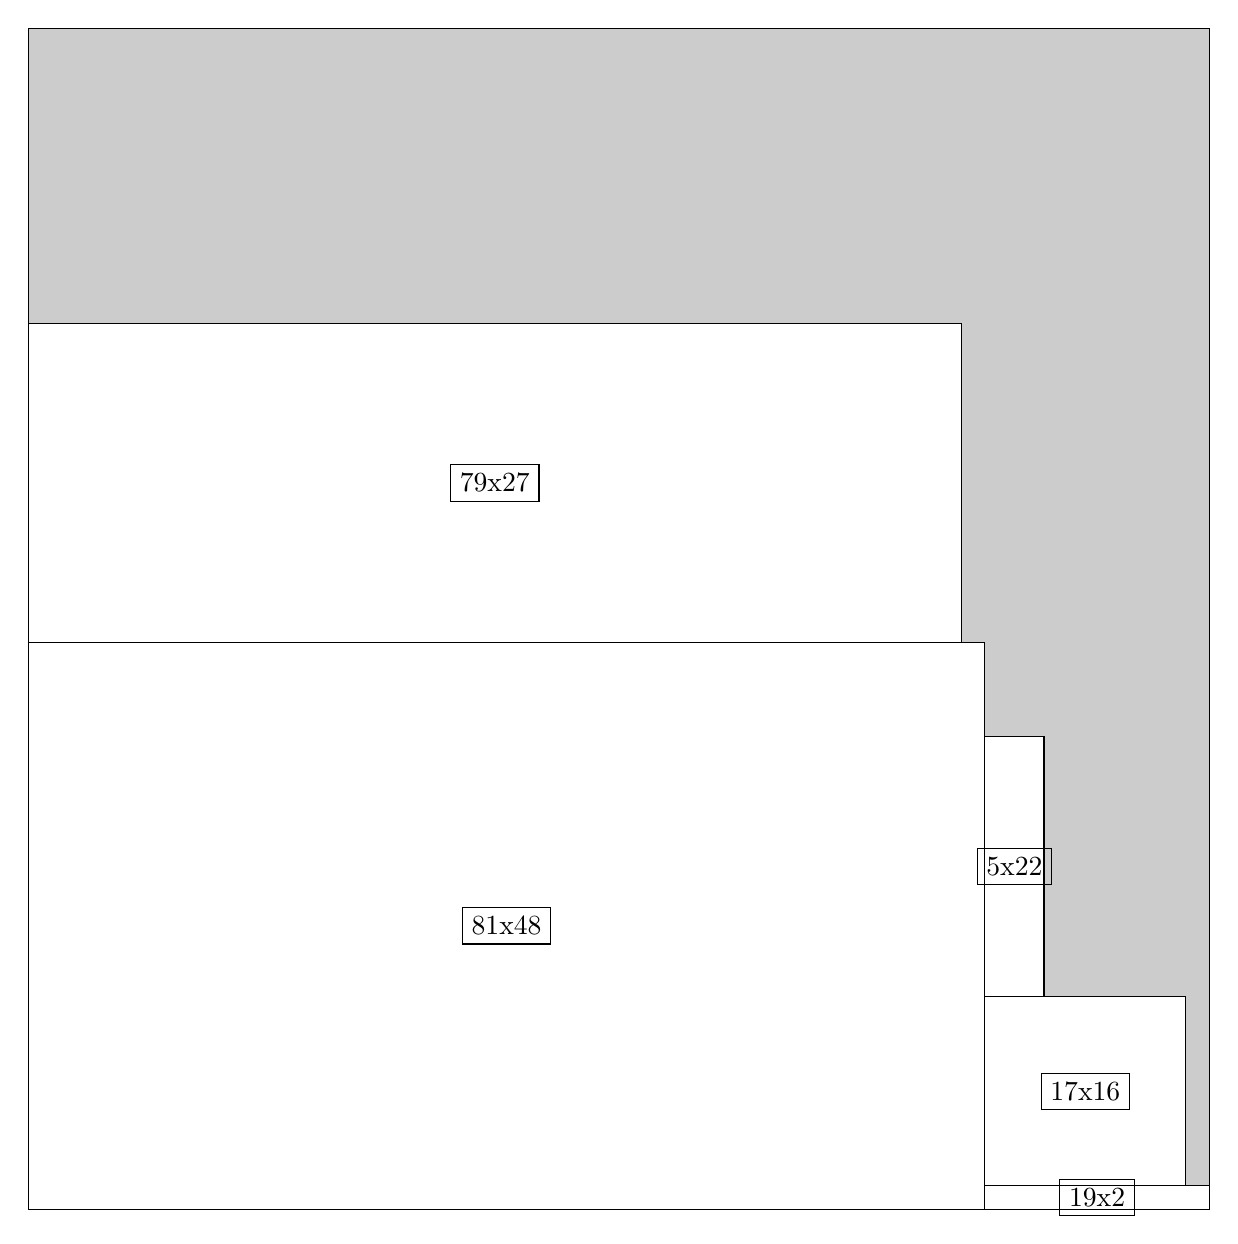
\begin{tikzpicture}[shorten >=1pt,scale=1.0,every node/.style={scale=1.0},->]
\tikzstyle{vertex}=[circle,fill=black!25,minimum size=14pt,inner sep=0pt]
\filldraw[fill=gray!40!white, draw=black] (0,0) rectangle (15.0,15.0);
\foreach \name/\x/\y/\w/\h in {81x48/0.0/0.0/12.15/7.199999999999999,79x27/0.0/7.199999999999999/11.85/4.05,17x16/12.15/0.3/2.55/2.4,5x22/12.15/2.6999999999999997/0.75/3.3,19x2/12.15/0.0/2.85/0.3}
\filldraw[fill=white!40!white, draw=black] (\x,\y) rectangle node[draw] (\name) {\name} ++(\w,\h);
\end{tikzpicture}


w =81 , h =48 , x =0 , y =0 , v =3888
\par
w =79 , h =27 , x =0 , y =48 , v =2133
\par
w =17 , h =16 , x =81 , y =2 , v =272
\par
w =5 , h =22 , x =81 , y =18 , v =110
\par
w =19 , h =2 , x =81 , y =0 , v =38
\par
\newpage


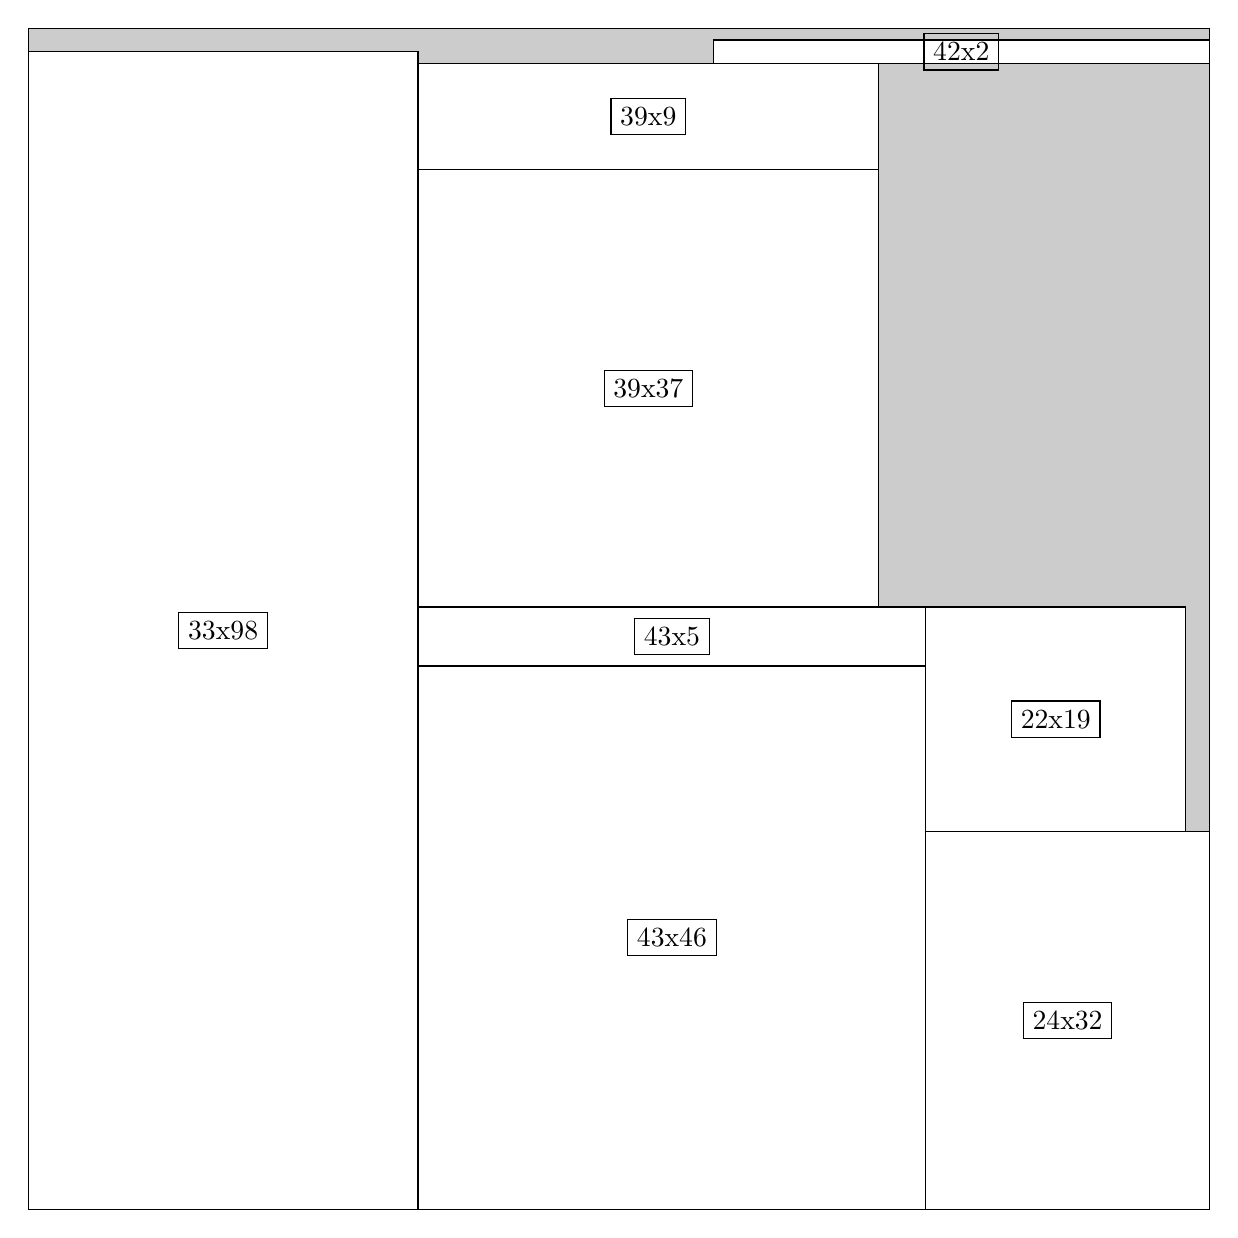
\begin{tikzpicture}[shorten >=1pt,scale=1.0,every node/.style={scale=1.0},->]
\tikzstyle{vertex}=[circle,fill=black!25,minimum size=14pt,inner sep=0pt]
\filldraw[fill=gray!40!white, draw=black] (0,0) rectangle (15.0,15.0);
\foreach \name/\x/\y/\w/\h in {33x98/0.0/0.0/4.95/14.7,43x46/4.95/0.0/6.45/6.8999999999999995,39x37/4.95/7.6499999999999995/5.85/5.55,24x32/11.4/0.0/3.5999999999999996/4.8,22x19/11.4/4.8/3.3/2.85,39x9/4.95/13.2/5.85/1.3499999999999999,43x5/4.95/6.8999999999999995/6.45/0.75,42x2/8.7/14.549999999999999/6.3/0.3}
\filldraw[fill=white!40!white, draw=black] (\x,\y) rectangle node[draw] (\name) {\name} ++(\w,\h);
\end{tikzpicture}


w =33 , h =98 , x =0 , y =0 , v =3234
\par
w =43 , h =46 , x =33 , y =0 , v =1978
\par
w =39 , h =37 , x =33 , y =51 , v =1443
\par
w =24 , h =32 , x =76 , y =0 , v =768
\par
w =22 , h =19 , x =76 , y =32 , v =418
\par
w =39 , h =9 , x =33 , y =88 , v =351
\par
w =43 , h =5 , x =33 , y =46 , v =215
\par
w =42 , h =2 , x =58 , y =97 , v =84
\par
\newpage


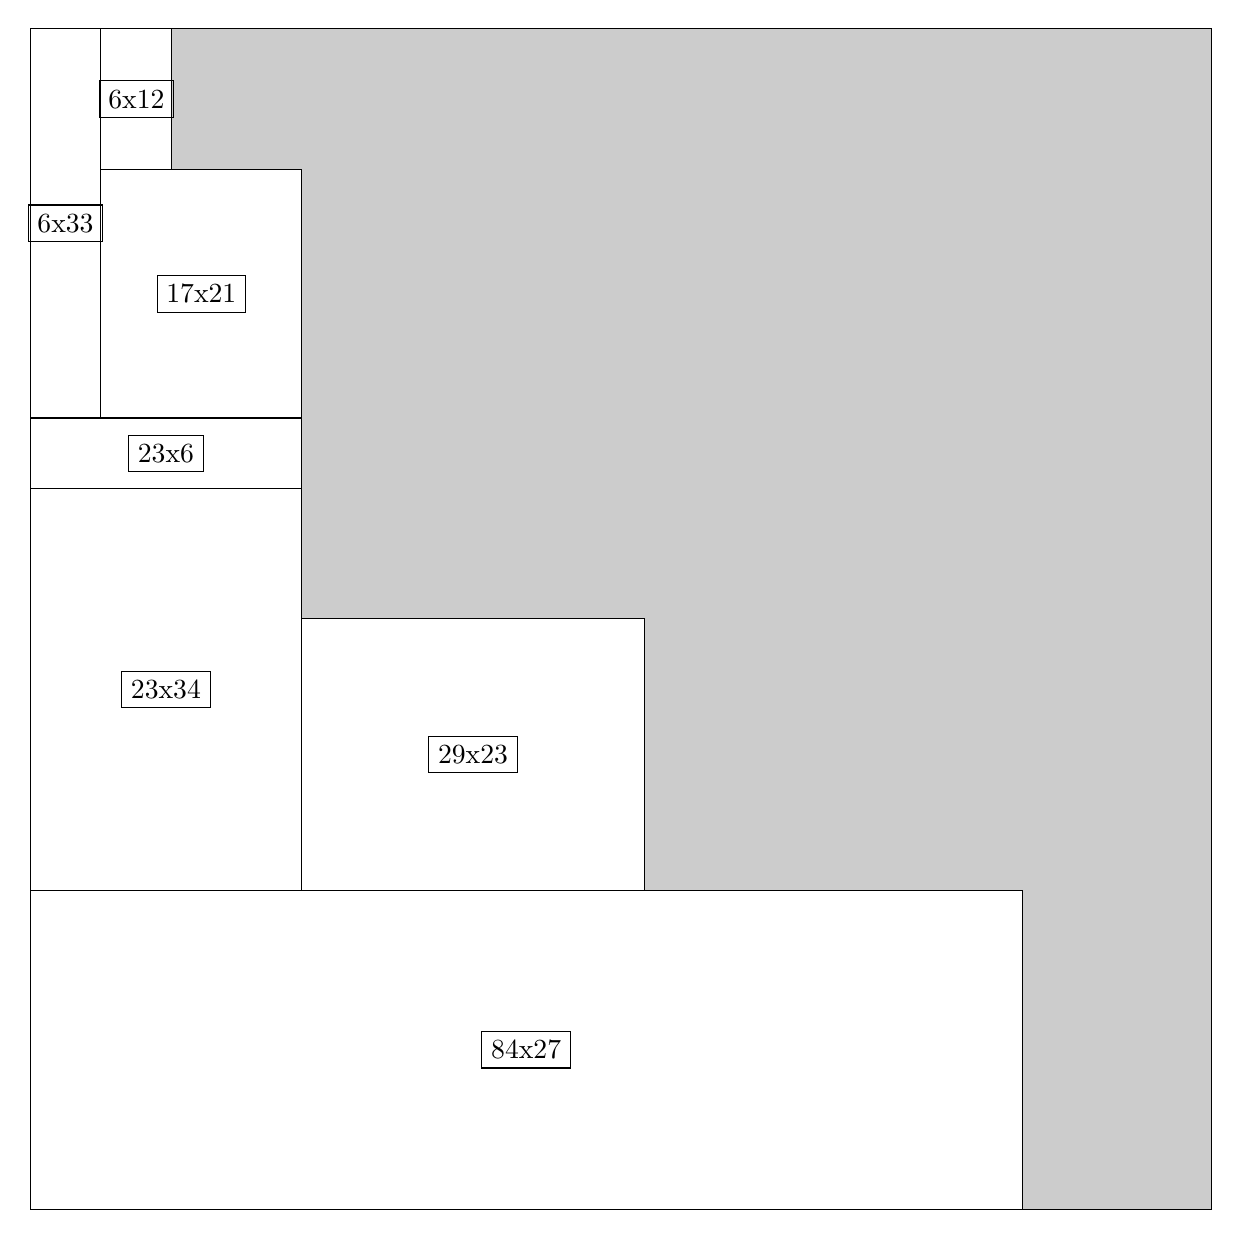
\begin{tikzpicture}[shorten >=1pt,scale=1.0,every node/.style={scale=1.0},->]
\tikzstyle{vertex}=[circle,fill=black!25,minimum size=14pt,inner sep=0pt]
\filldraw[fill=gray!40!white, draw=black] (0,0) rectangle (15.0,15.0);
\foreach \name/\x/\y/\w/\h in {84x27/0.0/0.0/12.6/4.05,23x34/0.0/4.05/3.4499999999999997/5.1,29x23/3.4499999999999997/4.05/4.35/3.4499999999999997,17x21/0.8999999999999999/10.049999999999999/2.55/3.15,6x33/0.0/10.049999999999999/0.8999999999999999/4.95,23x6/0.0/9.15/3.4499999999999997/0.8999999999999999,6x12/0.8999999999999999/13.2/0.8999999999999999/1.7999999999999998}
\filldraw[fill=white!40!white, draw=black] (\x,\y) rectangle node[draw] (\name) {\name} ++(\w,\h);
\end{tikzpicture}


w =84 , h =27 , x =0 , y =0 , v =2268
\par
w =23 , h =34 , x =0 , y =27 , v =782
\par
w =29 , h =23 , x =23 , y =27 , v =667
\par
w =17 , h =21 , x =6 , y =67 , v =357
\par
w =6 , h =33 , x =0 , y =67 , v =198
\par
w =23 , h =6 , x =0 , y =61 , v =138
\par
w =6 , h =12 , x =6 , y =88 , v =72
\par
\newpage


\end{document}